\section{Paper 5}
\subsection{\emph{"An End-to-End Multi-Task and Fusion CNN for Inertial-Based Gait Recognition"}}

\begin{frame}{INTRODUCTION}
    The gait recognition is an activity used in the medical, security and 
    authentication fields. The following paper shows a convolutional neural 
    network (CNN) which takes as input a series of inertial data, coming 
    from different sensors, and produces as output a prediction useful for 
    recognizing a subject.
    \begin{figure}[htbp]
        \centering
        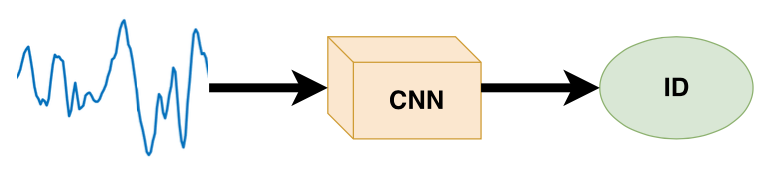
\includegraphics[width = 0.6 \linewidth]{images/paper5/usecase.png}
        \centering
        \caption{A preview of how the model works.}
        \label{fig:preview}
    \end{figure}
\end{frame}

\begin{frame}{RELATED WORK}
    Some methods have placed inertial sensors in different parts of the body 
    such as legs \footfullcite{0857651733}, hips \footfullcite{0857651732}, ankles, or even in objects such as bags and 
    pockets. Other methods \footfullcite{0857651736} directly use all the inertial sensors present in 
    the smartphone. In the proposed method, the data coming from the 
    different sensors are merged and sent to the network which will have the 
    task of predicting some tasks such as: {\bfseries{Identification}}, {\bfseries{age}} and {\bfseries{gender}} of 
    the subject.
\end{frame}

\begin{frame}{PROPOSED APPROACH - CNN Architecture}
    \begin{figure}[htbp]
        \centering
        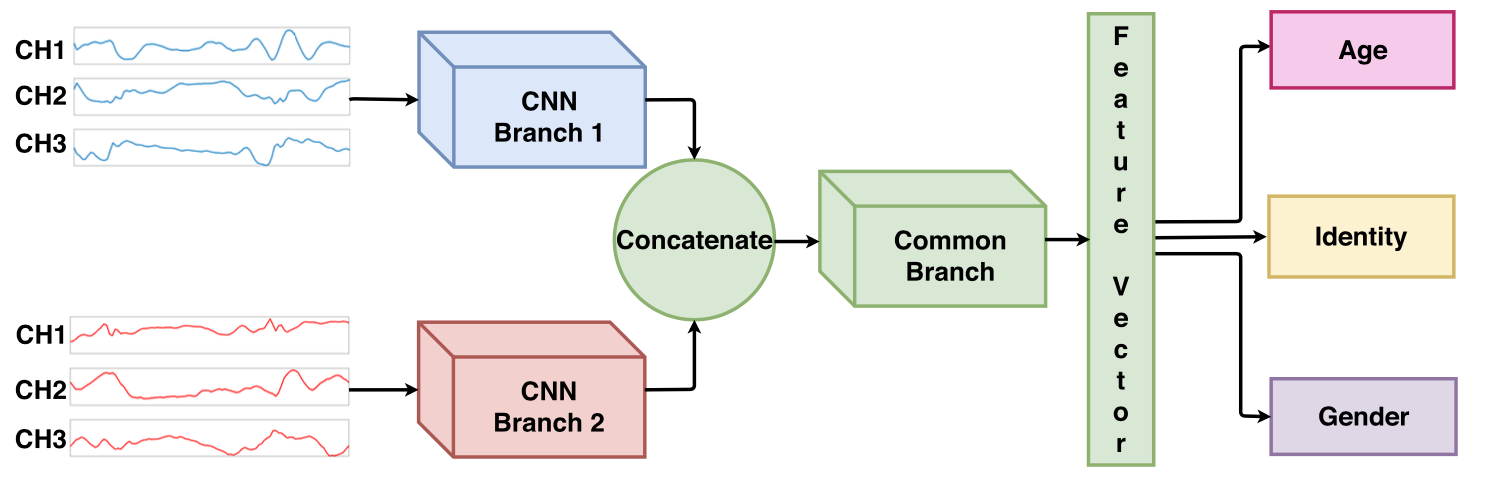
\includegraphics[width = 0.8 \linewidth]{images/paper5/architecture.png}
        \centering
        \caption{Pipeline for multi-task and multi-sensor learning in a gait-based system}
        \label{fig:pipeline}
    \end{figure}
    The network consists of two branches, one for each sensor (accelerometer 
    and gyroscope). The Input is split into 3 channels, 1 for each physical 
    size of the signal (axis x, y and z). After merging the data into a single 
    branch, the feature vector is extracted and then the three classes are 
    predicted. The data used are those present in the OU-ISIR dataset \small\footfullcite{0857651721}.
\end{frame}

\begin{frame}{PROPOSED APPROACH - Multi-Task}
    A network that manages different labels falls into the category of deep 
    multitask (\emph{DMT}) networks. To train this network, the sequence S of data 
    coming in input is splitted into $ s_i $ sub-sequences each of which will be 
    inserted in a tuple $ I = (s_i, y_i^m, y_1^1, ..., y_i^T) $ where $ y_i^m $ is the label of the 
    main task, $ y_i^t $, with $ t \in [1,T] $, is the label for each auxilary task. Both 
    the subsequences $ s_i $ and the tasks have their own loss function. The  total  
    accuracy  is  obtained  by combining the accuracies derived from the output 
    of each sub-sequence $ s_i $  of  the  input  S.
\end{frame}

\begin{frame}{PROPOSED APPROACH - Identity Authentication}
    Unlike the acknowledgment, the authentication problem aims to see if 
    two different inputs belong to the same subject. To do this, it is necessary 
    to calculate the Euclidean distances between the input data and the data 
    vectors present in the training set. Once this is done, the resulting vector 
    must be translated into probabilities that will be useful in order to 
    calculate two indices (Area Under Curve (AUC), Equal-Error-Rate 
    (EER)) that will be useful for evaluating the CNN network.
\end{frame}

\begin{frame}{EXPERIMENTS AND RESULTS - Gait recognition}
    For recognition, different types of experiments on different models and 
    their respective performances in terms of accuracy and F1-measure are 
    presented below.
    \begin{minipage}{\linewidth}
        \centering
        \begin{minipage}{0.45\linewidth}
            \begin{table}[h!]
            \centering
                \begin{adjustbox}{max width=\textwidth}
                \begin{tabular}{|c||ccc|c||ccc|c|}
                    \hline
                        & \multicolumn{4}{c||}{Acc} & \multicolumn{4}{c|}{F1-Score} \\
                    \hline
                        Architecture & Id & Age & Gender & Avg & Id & Age & Gender & Avg\\
                    \hline
                        SingleTask Accelerometer & 89.7 & 91.0 & 94.8 & 91.8 & 87.6 & 91.3 & 94.5 & 91.2\\
                        SingleTask Gyroscope& 89.1 & 89.1 & 94.4 & 90.9 & 87.5 & 89.7 & 94.4 & 90.5\\
                    \hline 
                \end{tabular}
                \end{adjustbox}
                \caption{Accuracy and F1-score (1 Task, 1 Sensor).}
                \label{table accuracy and F1 (1 Task - 1 Sensor)}
            \end{table}
            \centering
            \begin{table}[h!]
                \centering
                \begin{adjustbox}{max width=\textwidth}
                \begin{tabular}{|c||ccc|c||ccc|c|}
                    \hline
                        & \multicolumn{4}{c||}{Acc} & \multicolumn{4}{c|}{F1-Score} \\
                    \hline
                        Architecture & Id & Age & Gender & Avg & Id & Age & Gender & Avg\\
                    \hline
                        SingleTask Fusion & 94.2 & 95.0 & 95.6 & 94.9 & 93.5 & 95.0 & 95.6 & 94.7\\
                    \hline 
                \end{tabular}
                \end{adjustbox}
                \caption{Accuracy and F1-score (1 Task, + Sensor).}
                \label{table accuracy and F1 (1 Task, + Sensor)}
            \end{table}
        \end{minipage}
        \hspace{0.05\linewidth}
        \begin{minipage}{0.45\linewidth}
            \begin{figure}[htbp]
                \centering
                \begin{table}[h!]
                    \centering
                    \begin{adjustbox}{max width=\textwidth}
                    \begin{tabular}{|c||ccc|c||ccc|c|}
                        \hline
                            & \multicolumn{4}{c||}{Acc} & \multicolumn{4}{c|}{F1-Score} \\
                        \hline
                            Architecture & Id & Age & Gender & Avg & Id & Age & Gender & Avg\\
                        \hline
                            MultiTask Accelerometer & 90.9 & 93.3 & 95.9 & 93.4 & 89.1 & 93.3 & 95.9 & 92.8\\
                            MultiTask Gyroscope & 90.1 & 90.1 & 94.8 & 91.7 & 88.3 & 90.5 & 94.9 & 91.2\\
                        \hline 
                    \end{tabular}
                    \end{adjustbox}
                    \caption{Accuracy and F1-score (+ Task, 1 Sensor).}
                    \label{table accuracy and F1 (more Task - 1 Sensor)}
                \end{table}
                \centering
                \begin{table}[h!]
                    \centering
                    \begin{adjustbox}{max width=\textwidth}
                    \begin{tabular}{|c||ccc|c||ccc|c|}
                        \hline
                            & \multicolumn{4}{c||}{Acc} & \multicolumn{4}{c|}{F1-Score} \\
                        \hline
                            Architecture & Id & Age & Gender & Avg & Id & Age & Gender & Avg\\
                        \hline
                            MultiTask Fusion & \bfseries{94.8} & \bfseries{96.1} & \bfseries{97.7} & \bfseries{96.2} & \bfseries{93.8} & \bfseries{96.3} & \bfseries{97.7} & \bfseries{95.9}\\
                        \hline 
                    \end{tabular}
                    \end{adjustbox}
                    \caption{Accuracy and F1-score (1 Task, + Sensor).}
                    \label{table accuracy and F1 (+ Task, + Sensor)}
                \end{table}
            \end{figure}
        \end{minipage}
    \end{minipage}
\end{frame}

\begin{frame}{EXPERIMENTS AND RESULTS - Authentication}
    For identity authentication, on the other hand, the results shown in the table show that for this type of problem the single task model is better than the multi-task model. This happens because in this problem a single label (id) is required and not others. The introduction of other labels leads the multitask model to have worse accuracy than the single task model. The indices AUC (higher is better) and EER (lower is better) are calculated thanks to the probabilities obtained from the Euclidean distance vector.
    \begin{table}[h!]
        \centering
        \begin{adjustbox}{max width=\textwidth}
        \begin{tabular}{|c|cc|}
            \hline
            Architecture & EER & AUC\\
            \hline
            SingleTask Accelerometer & 1.47 & 99.91\\
            SingleTask Gyroscope & 2.50 & 99.80\\
            \hline
            MultiTask Accelerometer & 1.61 & 99.90\\
            MultiTask Gyroscope & 2.85 & 99.72\\
            \hline
            SingleTask Fusion & \bfseries{1.14} & \bfseries{99.93}\\
            \hline
            MultiTask Fusion & 1.34 & 99.92\\
            \hline
        \end{tabular}
        \end{adjustbox}
        \caption{Authentication accuracy.}
        \label{Authentication}
    \end{table}
\end{frame}

\begin{frame}{EXPERIMENTS AND RESULTS - State of the art Comparison}
    Comparing the proposed system with those already existing in the state 
    of the art, both for recognition and authentication, the performance, in 
    terms of accuracy, achieved outperforms those competitors.
        \begin{minipage}{\linewidth}
        \centering
        \begin{minipage}{0.45\linewidth}
            \begin{table}[h!]
                \centering
                \begin{adjustbox}{max width=\textwidth}
                \begin{tabular}{|c|ccc|c|}
                    \hline
                    CNN & Id & Age & Gender & Avg\\
                    \hline
                    AE-GDI-CC & 61.0 & - & - & -\\
                    Muaaz et al. & 63.5 & - & - & -\\
                    Ngo et al. & 70.2 & - & - & -\\
                    Wei et al. & 83.8 & - & - & - \\
                    \hline
                    MultiTask Fusion & \bfseries{94.8} & \bfseries{96.1} & \bfseries{97.7} & \bfseries{96.2}\\
                    \hline
                \end{tabular}
                \end{adjustbox}
                \caption{Gait recognition comparison with some methods.}
                \label{Gait comparison}
            \end{table}
        \end{minipage}
        \hspace{0.05\linewidth}
        \begin{minipage}{0.45\linewidth}
            \begin{table}[h!]
                \centering
                \begin{adjustbox}{max width=\textwidth}
                \begin{tabular}{|c|c|}
                    \hline
                    Approach & EER\\
                    \hline
                    Gafurov et al. & 15.8 \\
                    Derawi et al. & 14.3 \\
                    Rong et al. & 14.3 \\
                    Ngo et al. & 13.5 \\
                    Imp GDI + i-vector & 7.1 \\
                    NC GDI + i-vector & 5.6 \\
                    \hline
                    SingleTask Fusion & \bfseries{1.1}\\
                    \hline
                \end{tabular}
                \end{adjustbox}
                \caption{Authentication comparison with some methods.}
                \label{Authentication comparison}
            \end{table}
        \end{minipage}
    \end{minipage}
\end{frame}

\begin{frame}{CONCLUSIONS}
    As a final consideration, the model to be used, in the case of gait recognition, 
    is the one that merges the input information and adopts a multitask 
    approach. On the other hand, as regards the authentication problem, it has 
    been seen that it is better to use a singletask model.
\end{frame}